% Template file for a standard thesis
\documentclass[11pt,notitlepage]{isuthesis}
% notitlepage is used because \begin{abstract} uses titlepage by default, which resets the page numbers

\usepackage[pdftex]{graphicx}
% Standard, old-style thesis
\usepackage{isutraditional}   
\chaptertitle
% Old-style, thesis numbering down to subsubsection
\alternate
\usepackage{rotating}
% Bibliography without numbers or labels
%\usepackage{natbib}
% Use the following line if you want square brackets and numbering system
%\usepackage[square, numbers]{natbib}

\usepackage[sectionbib]{natbib}
\renewcommand{\bibfont}{\setstretch{1}\selectfont}
\setlength{\bibsep}{13.2pt}
\usepackage{chapterbib}

%\usepackage{chapterbib}
%\renewcommand\bibsection{\section*{\ref name}}
%\renewcommand\bibsection{\section*}
\renewcommand{\bibsection}{\section{References}}

%\bibliographystyle{apa}  % changed from apa, abbrv, unsrtnat
%\includeonly{titletoc,chapter1}
%Optional Package to add PDF bookmarks and hypertext links
\usepackage[pdftex,hypertexnames=false,linktocpage=true]{hyperref}
\hypersetup{colorlinks=true,linkcolor=blue,anchorcolor=blue,citecolor=blue,filecolor=blue,urlcolor=blue,bookmarksnumbered=true,pdfview=FitB}

%\usepackage{titletoc}
\usepackage{hyperref}

% \usepackage{subfig} %% Use this package instead of the subcaptions package for subfigures. Please see at the end of this file, an example of how to use the package.

\overfullrule=0pt
%%%%%%%%%%%%%%%%%%%%%

% The following piece of code removes extra space on the top of each chapter
%  that is default of latex report class documents

\usepackage{etoolbox}
\makeatletter
\patchcmd{\@makechapterhead}{50\p@}{0pt}{}{}
\patchcmd{\@makeschapterhead}{50\p@}{0pt}{}{}
\makeatother

%%%%%%%%%%%%%%%%%%%%%%%
%%%%%%%%%%%%%%%%%%%%%%%%%
% Removing Bold characters in the Table of Contents
% % Alternatively to this the isuthesis.cls file has been changed by default in the
% % line section \renewcommand{\l@chapter}[2]{\addpenalty{-\@highpenalty}....
%\titlecontents{chapter}
%[0pt]                                               % left margin
%{}%
%{\contentsmargin{0pt}                               % numbered entry format
%    \thecontentslabel\enspace%
%    \large}
%{\contentsmargin{0pt}\large}                        % unnumbered entry format
%{\titlerule*[.5pc]{.}\contentspage}                 % filler-page format (e.g dots)
%[]                                                  % below code (e.g vertical space)
%%%%%%%%%%%%%%%%%%%%%%%%%%

%%%%%%%%%%%%%%%%%%%%%%%%%%%%%%%
% In order to change space between the Table of contents items go to isuthesis.cls
% line  \renewcommand{\l@chapter}[2]{\addpenalty{-\@highpenalty}....
% change \vkip values

%%%%%%%%%%%%%%%%%%%%%%%%%%
%% This is to minimize orphan lines. Might not be possible to entirely remove them
% Method 1 of doing this
\widowpenalty100000
\clubpenalty100000

% Method 2 of doing this
\usepackage[all]{nowidow}
%%%%%%%%%%%%%%%%%%%%%%%%%%%

%%% control bibliography spacings
% \newlength{\bibitemsep}\setlength{\bibitemsep}{\baselineskip}
% % plus .05\baselineskip minus .05\baselineskip}
% \newlength{\bibparskip}\setlength{\bibparskip}{0pt}
% \let\oldthebibliography\thebibliography
% \renewcommand\thebibliography[1]{%
%   \oldthebibliography{#1}%
%   \setlength{\parskip}{\bibitemsep}%
%   \setlength{\itemsep}{\bibparskip}%
% }
% \usepackage{setspace}
% \setlength{\bibsep}{2sp}


%%%%%%%%%%%%%%%%%%%%%%%%%%%%%%%%%%
% %% aligning lof captions
% \usepackage{tocloft}

%%%%%%%%%%%%%%%%%%%%%%%%%%%%%%%%%%
%% Set the margins in the whole document
\geometry{letterpaper, left=1in, top=1in, right=1in, bottom=1in, includehead=true} 
%%%%%%%%%%%%%%%%%%%%%%%%%%%%%%%%%%

\usepackage{amssymb}
\usepackage[intoc, english]{nomencl}

\begin{document}
\DeclareGraphicsExtensions{.jpg,.pdf,.mps,.png}
%\begin{singlespace}
\def\@makechapterheada{\vspace*{-2cm}\titlepage} % in order to reduce the space between margin and heading in titlepage
% Template Titlepage File
% Please choose appropriate options for Master's thesis, Doctoral dissertations, and creative components. Please read the comments to make an informed choice

\@makechapterheada\titlepage  % using definition from thesis.tex reduce the space between margin and heading in titlepage
\title{This is the title of a thesis
submitted to Iowa State University\\
Note that only the first letter of
the first word and proper names
are capitalized}

\author{Wilbur Terrance Johnson}

%%%%%%%%%%%%%%%%%%%
%% Master of Science options. 
%% CC will have a couple of changes mentioned near the end of this file.

\degree{MASTER OF SCIENCE}
\major{Human Development and Family Studies (Marriage and Family Therapy)}
% Use the following line for co-majors (usually used with doctoral dissertations)
%\comajors{Statistics; Computer Science}{}

\level{master's}
\mprof{Susan D. Ross}
% In case of co majors please comment out the mprof line above and use the following two lines of mprofs and cmprofs to defines the two co-major profs
%\mprofs{ABC}
%\cmprofs{DEF}

\members{Mary Jones \\ Bjork Petersen \\}
\disclaimertitlepage{The student author, whose presentation of the scholarship herein was approved by the program of study committee, is solely responsible for the content of this dissertation/thesis. The Graduate College will ensure this dissertation/thesis is globally accessible and will not permit alterations after a degree is conferred.}
%{The student author and the program of study committee are solely responsible for the content of this dissertation/thesis. The Graduate College will ensure this dissertation/thesis is globally accessible and will not permit alterations after a degree is conferred.}


%%%%%%%%%%%%%%%%%%%%%%%%%%%%
% Doctor of Philosophy options
% If co-majors select only co-major options as described and skip other options like \major, \mprof and make sure committee members are appropriately included.


% Add these additional lines for a Doctoral Dissertation
%\degree{DOCTOR OF PHILOSOPHY}
% \major{Human Development and Family Studies (Marriage and Family Therapy)}
% Use the following line for co-majors (usually used with doctoral dissertations)
%\comajors{Statistics; Computer Science}{}
%\level{doctoral}
%\mprof{Susan D. Ross}
% In case of co majors please comment out the mprof line above and use the following two lines of mprofs and cmprofs to defines the two co-major profs
%\mprofs{ABC}
%\cmprofs{DEF}

%\format{dissertation}
%\committee{4}
%\members{Mary Jones \\ Bjork Petersen \\ Sam Anders \\ Harold Jones}
%\disclaimertitlepage{The student author, whose presentation of the scholarship herein was approved by the program of study committee, is solely responsible for the content of this dissertation/thesis. The Graduate College will ensure this dissertation/thesis is globally accessible and will not permit alterations after a degree is conferred.}

%%%%%%%%%%%%%%
% Creative component: lines to add / remove
% Add these additional lines for a Creative Component
% - also comment out the \maketitle command
%\format{Creative Component}
%\submit{the graduate faculty}

\notice
\maketitle

%\end{singlespace}

% Left-justified setting for all sections including
% dedication, nomenclature, acknowledgement, abstract and all chapters
% Re-position the two lines below will change all the section
% being compiled after those two lines
\raggedright
\parindent 0.25 in % set all paragraphs in the document to have indent

% Optional thesis dedication
\chapter*{DEDICATION}

I would like to dedicate this thesis to my wife Glenda and
to my daughter Alice without whose support I would not have
been able to complete this work.



% Table of Contents, List of Tables and List of Figures
{
\pdfbookmark[1]{TABLE OF CONTENTS}{table}
\tableofcontents
}
%%%%%%%%%%%%%%%%%%%%%%%%%%%%%%%%%%%%%%%%%
%% The line below adds the word "Page" over the page numbers in TOC, LOT, LOF
\addtocontents{toc}{~\hfill\textbf{Page}\par}
\addtocontents{lot}{~\hfill\textbf{Page}\par}
\addtocontents{lof}{~\hfill\textbf{Page}\par}
%%
\addtocontents{toc}{\def\protect\@chapapp{}} \cleardoublepage \phantomsection
\pagebreak
\addcontentsline{toc}{chapter}{LIST OF TABLES}
%%%%%%%%%%%%%%%%%%%%%%%%%%%%%%%%%%%%%%%%%
\listoftables
\cleardoublepage \phantomsection \addcontentsline{toc}{chapter}{LIST OF FIGURES}
%%%%%%%%%%%%%%%%%%%%%%%%%%%%%%%%%%%%%%%%%
\listoffigures

%Optional Nomenclature
\cleardoublepage \phantomsection
\makenomenclature
\renewcommand{\nomname}{NOMENCLATURE}
%\specialchapt{NOMENCLATURE}

%\mbox{}
\renewcommand\nomgroup[1]{%
  \item[\bfseries
  \ifstrequal{#1}{P}{Physics Constants}{%
  \ifstrequal{#1}{N}{Number Sets}{%
  \ifstrequal{#1}{O}{Other Symbols}{}}}%
]}

\nomenclature[P]{$c$}{Speed of light in a vacuum inertial system}
\nomenclature[P]{$h$}{Plank Constant}
\nomenclature[P]{$g$}{Gravitational Constant}
\nomenclature[N]{$\mathbb{R}$}{Real Numbers}
\nomenclature[N]{$\mathbb{C}$}{Complex Numbers}
\nomenclature[N]{$\mathbb{H}$}{Quaternions}
\nomenclature[O]{$V$}{Constant Volume}
\nomenclature[O]{$\rho$}{Friction Index}

\renewcommand{\nompreamble}{The nomenclature for your dissertation or thesis is optional. This list may be placed in
the following places: as the last preliminary page, before the Reference section, or as an Appendix. The heading is bold if other major headings are bold, and the list is in the same font size and style as text. Nomenclature should follow a two-column format with the term in the left
column and its definition or description within the right column.}

\printnomenclature

% The following link has more tweaks, tips and tricks on how to setup nomenclatures: https://www.overleaf.com/learn/latex/Nomenclatures

% Comment out the next line if NOT using chaptertitle
\addtocontents{toc}{\def\protect\@chapapp{CHAPTER\ }}

%Optional Acknowledgements
\cleardoublepage \phantomsection
\specialchapt{ACKNOWLEDGMENTS}

I would like to take this opportunity to express my thanks to those
who helped me with various aspects of conducting research and the writing
of this thesis.
First and foremost, Dr. Susan D. Ross for her guidance, patience and support
throughout this research and the writing of this thesis.
Her insights and words of encouragement have often inspired me and renewed
my hopes for completing my graduate education.
I would also like to thank my committee members for their efforts
and contributions to this work: Dr. August Tanner and
Dr. Lewis Hargrave.
I would additionally like to thank
Dr. Tanner for his guidance throughout the initial stages of my
graduate career and Dr. Hargrave for his inspirational teaching style.

%Optional thesis abstract
\cleardoublepage \phantomsection
\specialchapt{ABSTRACT}

This is the text of my abstract that is part of the thesis itself.
The abstract describes the work in general and the heading and style
match the rest of the document.

\newpage
\pagenumbering{arabic}

% Create body using the info from _bookdown.yml
%\textbackslash{}

\chapter{GENERAL INTRODUCTION}

This chapter will have the introduction to your thesis as a whole.

This is the opening paragraph to my thesis which
explains in general terms the concepts and hypothesis
which will be used in my thesis.

With more general information given here than really
necessary.

\begin{center}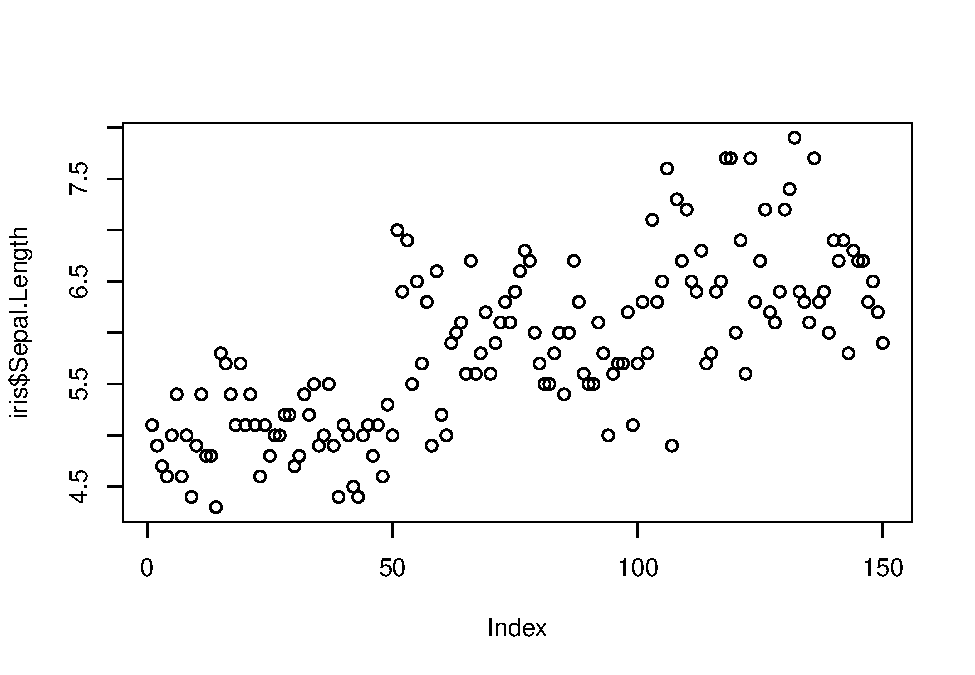
\includegraphics{thesis_files/figure-latex/unnamed-chunk-1-1} \end{center}

\section{Overview}

Here initial concepts and conditions are explained and
several hypothesis are mentioned in brief.

\subsection{Hypothesis}

Here one particular hypothesis is explained in depth
and is examined in the light of current literature.

\subsubsection{Parts of the hypothesis}

Here one particular part of the hypothesis that is
currently being explained is examined and particular
elements of that part are given careful scrutiny.

\subsection{Second Hypothesis}

Here one particular hypothesis is explained in depth
and is examined in the light of current literature.

\subsubsection{Parts of the second hypothesis}

Here one particular part of the hypothesis that is
currently being explained is examined and particular
elements of that part are given careful scrutiny
\cite{allen}, \cite{bruner}, \cite{prime-number-theorem} abcd.

\section{Criteria Review}

Here certain criteria are explained thus eventually
leading to a foregone conclusion.

\bibliographystyle{apa}
\bibliography{master_bib}

\textbackslash{}

\chapter{PAPER 1 TITLE GOES HERE}

\label{polymer_fibers}

\begin{center}
    Authors and Affiliations \\
    Modified from a manuscript to be submitted to/ under review/ published in \textit{Name of the Journal} 
\end{center}

\section{Abstract}

This is the text of my abstract that is part of the thesis itself.
The abstract describes the work in the first paper general. You can use the same abstract as your paper here.

\section{Overview}

The construct of this section or any further section is same as the authors paper.
This is the opening paragraph to my thesis which
explains in general terms the concepts and hypothesis
which will be used in my thesis.

With more general information given here than really
necessary.

\section{Introduction}

Here initial concepts and conditions are explained and
several hypothesis are mentioned in brief.

\cite{allen}, \cite{bruner} and \cite{cox}
did the initial work in this area. But in Struss' work {[}\cite{struss}{]}
the definitive model is seen.

\subsection{Hypothesis}

Here one particular hypothesis is explained in depth
and is examined in the light of current literature.

\subsubsection{Parts of the hypothesis}

Here one particular part of the hypothesis that is
currently being explained is examined and particular
elements of that part are given careful scrutiny.

\subsection{Second Hypothesis}

Here one particular hypothesis is explained in depth
and is examined in the light of current literature.

\subsubsection{Parts of the second hypothesis}

Here one particular part of the hypothesis that is
currently being explained is examined and particular
elements of that part are given careful scrutiny.

\section{Criteria Review}

Here certain criteria are explained thus eventually
leading to a foregone conclusion.

\section{Conclusion}\label{conclusion}

The conclusion of the paper goes here.
\cite{cox}
\cite{Ancey1996}, \cite{RR73}
\cite{Aup91}, \cite{Dou72}

\section{Appendix A: Appendix A Title Goes Here After The Colon}

If there is an appendix that needs to go with the paper it can be as a section \cite{Aup91}

\subsection{Procedure details}

Details of the paper specific appendix procedures

\section{Appendix B: Appendix B Title Goes Here After The Colon}

If there is an appendix that needs to go with the paper it can be as a section \cite{Aup91}

\subsection{Procedure details}

Details of the paper specific appendix procedures

\chapter{PAPER 2 TITLE GOES HERE}

\begin{center}
    Authors and Affiliations \\
    Modified from a manuscript to be submitted to/ under review/ published in \textit{Name of the Journal} 
\end{center}

\section{Abstract}

This is the text of my abstract that is part of the thesis itself.
The abstract describes the work in the first paper general. You can use the same abstract as your paper here.

\section{Overview}

The construct of this section or any further section is same as the authors paper.
This is the opening paragraph to my thesis which
explains in general terms the concepts and hypothesis
which will be used in my thesis.

With more general information given here than really
necessary.

\section{Introduction}

Here initial concepts and conditions are explained and
several hypothesis are mentioned in brief.

\cite{allen}, \cite{bruner} and \cite{cox}
did the initial work in this area. But in Struss' work {[}\cite{struss}{]}
the definitive model is seen.

\subsection{Hypothesis}

Here one particular hypothesis is explained in depth
and is examined in the light of current literature.

\subsubsection{Parts of the hypothesis}

Here one particular part of the hypothesis that is
currently being explained is examined and particular
elements of that part are given careful scrutiny.

\subsection{Second Hypothesis}

Here one particular hypothesis is explained in depth
and is examined in the light of current literature.

\subsubsection{Parts of the second hypothesis}

Here one particular part of the hypothesis that is
currently being explained is examined and particular
elements of that part are given careful scrutiny.

\addtocontents{toc}{\protect\newpage}

\%\% Remove this if needed, this lines forces the lines of the TOC starting with the below sub-heading ``Critical Review'' to go to the next page. Remove this formatting line as it will be required only if you want to force a table of contents entry to the next page along with the other subsequent entries.

\section{Criteria Review}

Here certain criteria are explained thus eventually
leading to a foregone conclusion.

\section{Conclusion}\label{Conclusion1}

The conclusion of the paper goes here.

\cite{allen}, \cite{bruner},
\cite{Hal82},
\cite{Rud73}, \cite{Con90},
\cite{Con78}, \cite{KR83},
\cite{KR86}

\section{Appendix: Appendix Title Goes Here}

If there is an appendix that needs to go with the paper it can be as a section \cite{Aup91}

\subsection{Procedure details}

Details of the paper specific appendix procedures

\chapter{PAPER 3 TITLE GOES HERE}

\begin{center}
    Authors and Affiliations \\
    Modified from a manuscript to be submitted to/ under review/ published in \textit{Name of the Journal} 
\end{center}

\section{Abstract}

This is the text of my abstract that is part of the thesis itself.
The abstract describes the work in the first paper general. You can use the same abstract as your paper here.

\section{Methods and procedures}

This is the opening paragraph to my thesis which
explains in general terms the concepts and hypothesis
which will be used in my thesis.

With more general information given here than really
necessary.

\section{Introduction}

Here initial concepts and conditions are explained and
several hypothesis are mentioned in brief.

As can be seen in Table\textasciitilde{}\ref{nothing} it is truly
obvious what I am saying is true.

\begin{table}[h!tb] \centering
\isucaption[This table shows a standard empty table. Please check the code caption for extended instructions]{This table shows a standard empty table. In case of long captions, we want to use the long caption as the description to the table and image but not use it in the table of contents and list of figures/ tables. In order to do this, there are two captions which have been provided, remove the first square bracket options if there is only one small caption. You can use citations like this too \cite{Enf87}}
\label{nothing}

\vspace{ 2 in}
\end{table}

\subsection{Hypothesis}

Here one particular hypothesis is explained in depth
and is examined in the light of current literature.

This can also be seen in Figure\textasciitilde{}\ref{moon} that the
rest is obvious.

\begin{figure}[h!tb] \centering

\vspace{ 2 in}
\isucaption{This table shows a standard empty figure}
\label{moon}
\end{figure}

\subsubsection{Parts of the hypothesis}

Here one particular part of the hypothesis that is
currently being explained is examined and particular
elements of that part are given careful scrutiny.

\subsection{Second Hypothesis}

Here one particular hypothesis is explained in depth
and is examined in the light of current literature.

\subsubsection{Parts of the second hypothesis}

Here one particular part of the hypothesis that is
currently being explained is examined and particular
elements of that part are given careful scrutiny.

Here certain criteria are explained thus eventually
leading to a foregone conclusion as can be seen in
Table \ref{nevermore}.

\begin{table}[h!tb] \centering
\setlength{\captionwidth}{3.5 in}
\isucaption{This table shows a standard empty table with a limited caption width}
\label{nevermore}

\vspace{ 2 in}
\end{table}

\section{Results}

Include any results

\section{Conclusion}\label{conclusion2}

The conclusion of the paper goes here.

\cite{Rea85}
\cite{Enf87}, \cite{Dau75}
\cite{KPS75}

\section{Appendix: Appendix Title Goes Here}

If there is an appendix that needs to go with the paper it can be as a section \cite{Aup91}

\subsection{Procedure details}

Details of the paper specific appendix procedures

\chapter{PAPER 4 TITLE GOES HERE}

\begin{center}
    Authors and Affiliations \\
    Modified from a manuscript to be submitted to/ under review/ published in \textit{Name of the Journal} 
\end{center}

\section{Abstract}

This is the text of my abstract that is part of the thesis itself.
The abstract describes the work in the first paper general. You can use the same abstract as your paper here.

This is the opening paragraph to my thesis which
explains in general terms the concepts and hypothesis
which will be used in my thesis.

With more general information given here than really
necessary.

\section{Introduction}

Here initial concepts and conditions are explained and
several hypothesis are mentioned in brief.

Of course, data on this as seen in Table\textasciitilde{}\ref{data}
is few and far between.

\begin{table}[h!tb] \centering
\isucaption{Moon Data}
\label{data}
<!-- % Use: \begin{tabular{|lcc|} to put table in a box -->
\begin{tabular}{lcc} \hline
\textbf{Element} & \textbf{Control} & \textbf{Experimental} \\ \hline
Moon Rings & 1.23 & 3.38 \\
Moon Tides & 2.26 & 3.12 \\
Moon Walk & 3.33 & 9.29 \\ \hline
\end{tabular}
\end{table}

\subsection{Hypothesis}

Here one particular hypothesis is explained in depth
and is examined in the light of current literature.

Or graphically as seen in Figure\textasciitilde{}\ref{mgraph}
it is certain that my hypothesis is true.

\begin{figure}[h!tb] \centering

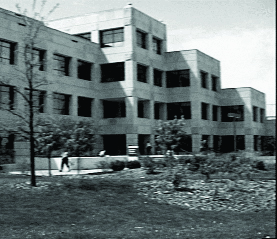
\includegraphics{Images/dc5}

\isucaption{Durham Centre}
\label{mgraph}
\end{figure}

\subsubsection{Parts of the hypothesis}

Here one particular part of the hypothesis that is
currently being explained is examined and particular
elements of that part are given careful scrutiny.

\subsection{Second Hypothesis}

Here one particular hypothesis is explained in depth
and is examined in the light of current literature.

\subsubsection{Parts of the second hypothesis}

Here one particular part of the hypothesis that is
currently being explained is examined and particular
elements of that part are given careful scrutiny.

\section{Criteria Review}

Here certain criteria are explained thus eventually
leading to a foregone conclusion.

\section{Results}

\section{Conclusion}\label{conclusion3}

The conclusion of the paper goes here.

\section{Appendix: Appendix title goes here}

If there is an appendix that needs to go with the paper it can be as a section \cite{Aup91}

\subsection{Procedure details}

Details of the paper specific appendix procedures

\cite{Rad87}
\cite{MOR91}, \cite{Lom73}
\cite{Lom91}, \cite{Lom92}
\cite{dB59}

\chapter{GENERAL CONCLUSION}
\label{future-work}

This is the opening paragraph to my thesis which
explains in general terms the concepts and hypothesis
which will be used in my thesis.

With more general information given here than really
necessary.

\section{Summary And Discussion}

Here initial concepts and conditions are explained and
several hypothesis are mentioned in brief.

\subsection{Hypothesis}

Here one particular hypothesis is explained in depth
and is examined in the light of current literature.

As can be seen in Table\textasciitilde{}\ref{nothingelse} it is
truly obvious what I am saying is true.

\begin{sidewaystable} \centering
\isucaption{This table shows almost nothing but is a
sideways table and takes up a whole page by itself}
\label{nothingelse}
% Use: \begin{tabular{|lcc|} to put table in a box
\begin{tabular}{lcc} \hline
\textbf{Element} & \textbf{Control} & \textbf{Experimental} \\ \hline
Moon Rings & 1.23 & 3.38 \\
Moon Tides & 2.26 & 3.12 \\
Moon Walk & 3.33 & 9.29 \\ \hline
\end{tabular}
\end{sidewaystable}

\subsubsection{Parts of the hypothesis}

Here one particular part of the hypothesis that is
currently being explained is examined and particular
elements of that part are given careful scrutiny. \cite{allen}, \cite{bruner}, \cite{struss}

%% Chapter 1 of the Thesis Template File
\chapter{GENERAL INTRODUCTION}
This chapter will have the introduction to your thesis as a whole.

This is the opening paragraph to my thesis which
explains in general terms the concepts and hypothesis
which will be used in my thesis.

With more general information given here than really
necessary.

\section{Overview}

Here initial concepts and conditions are explained and
several hypothesis are mentioned in brief.

\subsection{Hypothesis}

Here one particular hypothesis is explained in depth
and is examined in the light of current literature.

\subsubsection{Parts of the hypothesis}

Here one particular part of the hypothesis that is 
currently being explained is examined and particular
elements of that part are given careful scrutiny.

% Below \subsubsection
% Sectional commands: \paragraph and \subparagraph may also be used

\subsection{Second Hypothesis}

Here one particular hypothesis is explained in depth
and is examined in the light of current literature.

\subsubsection{Parts of the second hypothesis}

Here one particular part of the hypothesis that is 
currently being explained is examined and particular
elements of that part are given careful scrutiny
\cite{allen}, \cite{bruner}, \cite{prime-number-theorem} abcd. 

\section{Criteria Review}

Here certain criteria are explained thus eventually
leading to a foregone conclusion.

%\bibliographystyle{acm} % use for numbered citations along with options given in preamble. Look at the main thesis.tex file
\bibliographystyle{apa}
\bibliography{master_bib}

% \section{Bibliography}
% \bibliographystyle{apa}
% % \vspace{-20pt}
% \begingroup
%     \setlength{\bibsep}{13.2pt}
%     \linespread{1}\selectfont
%     \bibliography{master_bib}
% \endgroup
% \clearpage
% \pagebreak

%% Options for packages loaded elsewhere
\PassOptionsToPackage{unicode}{hyperref}
\PassOptionsToPackage{hyphens}{url}
%
\documentclass[
]{article}
\usepackage{lmodern}
\usepackage{amssymb,amsmath}
\usepackage{ifxetex,ifluatex}
\ifnum 0\ifxetex 1\fi\ifluatex 1\fi=0 % if pdftex
  \usepackage[T1]{fontenc}
  \usepackage[utf8]{inputenc}
  \usepackage{textcomp} % provide euro and other symbols
\else % if luatex or xetex
  \usepackage{unicode-math}
  \defaultfontfeatures{Scale=MatchLowercase}
  \defaultfontfeatures[\rmfamily]{Ligatures=TeX,Scale=1}
\fi
% Use upquote if available, for straight quotes in verbatim environments
\IfFileExists{upquote.sty}{\usepackage{upquote}}{}
\IfFileExists{microtype.sty}{% use microtype if available
  \usepackage[]{microtype}
  \UseMicrotypeSet[protrusion]{basicmath} % disable protrusion for tt fonts
}{}
\makeatletter
\@ifundefined{KOMAClassName}{% if non-KOMA class
  \IfFileExists{parskip.sty}{%
    \usepackage{parskip}
  }{% else
    \setlength{\parindent}{0pt}
    \setlength{\parskip}{6pt plus 2pt minus 1pt}}
}{% if KOMA class
  \KOMAoptions{parskip=half}}
\makeatother
\usepackage{xcolor}
\IfFileExists{xurl.sty}{\usepackage{xurl}}{} % add URL line breaks if available
\IfFileExists{bookmark.sty}{\usepackage{bookmark}}{\usepackage{hyperref}}
\hypersetup{
  hidelinks,
  pdfcreator={LaTeX via pandoc}}
\urlstyle{same} % disable monospaced font for URLs
\usepackage[margin=1in]{geometry}
\usepackage{graphicx,grffile}
\makeatletter
\def\maxwidth{\ifdim\Gin@nat@width>\linewidth\linewidth\else\Gin@nat@width\fi}
\def\maxheight{\ifdim\Gin@nat@height>\textheight\textheight\else\Gin@nat@height\fi}
\makeatother
% Scale images if necessary, so that they will not overflow the page
% margins by default, and it is still possible to overwrite the defaults
% using explicit options in \includegraphics[width, height, ...]{}
\setkeys{Gin}{width=\maxwidth,height=\maxheight,keepaspectratio}
% Set default figure placement to htbp
\makeatletter
\def\fps@figure{htbp}
\makeatother
\setlength{\emergencystretch}{3em} % prevent overfull lines
\providecommand{\tightlist}{%
  \setlength{\itemsep}{0pt}\setlength{\parskip}{0pt}}
\setcounter{secnumdepth}{-\maxdimen} % remove section numbering

\author{}
\date{\vspace{-2.5em}}

\begin{document}

\chapter{PAPER 1 TITLE GOES HERE}

\label{polymer_fibers}

\begin{center}
    Authors and Affiliations \\
    Modified from a manuscript to be submitted to/ under review/ published in \textit{Name of the Journal} 
\end{center}

\section{Abstract}

This is the text of my abstract that is part of the thesis itself. The
abstract describes the work in the first paper general. You can use the
same abstract as your paper here.

\section{Overview}

The construct of this section or any further section is same as the
authors paper. This is the opening paragraph to my thesis which explains
in general terms the concepts and hypothesis which will be used in my
thesis.

With more general information given here than really necessary.

\section{Introduction}

Here initial concepts and conditions are explained and several
hypothesis are mentioned in brief.

\cite{allen}, \cite{bruner} and \cite{cox} did the initial work in this
area. But in Struss' work {[}\cite{struss}{]} the definitive model is
seen.

\subsection{Hypothesis}

Here one particular hypothesis is explained in depth and is examined in
the light of current literature.

\subsubsection{Parts of the hypothesis}

Here one particular part of the hypothesis that is currently being
explained is examined and particular elements of that part are given
careful scrutiny.

\subsection{Second Hypothesis}

Here one particular hypothesis is explained in depth and is examined in
the light of current literature.

\subsubsection{Parts of the second hypothesis}

Here one particular part of the hypothesis that is currently being
explained is examined and particular elements of that part are given
careful scrutiny.

\section{Criteria Review}

Here certain criteria are explained thus eventually leading to a
foregone conclusion.

\section{Conclusion}\label{conclusion}

The conclusion of the paper goes here. \cite{cox} \cite{Ancey1996},
\cite{RR73} \cite{Aup91}, \cite{Dou72}

\bibliographystyle{apa}
\bibliography{master_bib}

\section{Appendix A: Appendix A Title Goes Here After The Colon}

If there is an appendix that needs to go with the paper it can be as a
section \cite{Aup91}

\subsection{Procedure details}

Details of the paper specific appendix procedures

\section{Appendix B: Appendix B Title Goes Here After The Colon}

If there is an appendix that needs to go with the paper it can be as a
section \cite{Aup91}

\subsection{Procedure details}

Details of the paper specific appendix procedures

\end{document}

%\chapter{PAPER 2 TITLE GOES HERE}
%\label{polymer_fibers}

\begin{center}
    Authors and Affiliations \\
    Modified from a manuscript to be submitted to/ under review/ published in \textit{Name of the Journal} 
\end{center}

\section{Abstract}
This is the text of my abstract that is part of the thesis itself.
The abstract describes the work in the first paper general. You can use the same abstract as your paper here.

%\pagebreak %remove if needed

% Please include sections as the paper has, some of the following sections are meant as examples of what can be done, the bibliography should be made as given

\section{Overview}

The  construct of this section or any further section is same as the authors paper.
This is the opening paragraph to my thesis which
explains in general terms the concepts and hypothesis
which will be used in my thesis.

With more general information given here than really
necessary.

\section{Introduction}

Here initial concepts and conditions are explained and
several hypothesis are mentioned in brief.

\cite{allen}, \cite{bruner} and \cite{cox}
did the initial work in this area. But in Struss' work [\cite{struss}]
the definitive model is seen.

\subsection{Hypothesis}

Here one particular hypothesis is explained in depth
and is examined in the light of current literature.

\subsubsection{Parts of the hypothesis}

Here one particular part of the hypothesis that is 
currently being explained is examined and particular
elements of that part are given careful scrutiny.

% Below \subsubsection
% Sectional commands: \paragraph and \subparagraph may also be used

\subsection{Second Hypothesis}

Here one particular hypothesis is explained in depth
and is examined in the light of current literature.

\subsubsection{Parts of the second hypothesis}

Here one particular part of the hypothesis that is 
currently being explained is examined and particular
elements of that part are given careful scrutiny.

\addtocontents{toc}{\protect\newpage} %% Remove this if needed, this lines forces the lines of the TOC starting with the below sub-heading "Critical Review" to go to the next page. Remove this formatting line as it will be required only if you want to force a table of contents entry to the next page along with the other subsequent entries.

\section{Criteria Review}

Here certain criteria are explained thus eventually
leading to a foregone conclusion.

\section{Conclusion}\label{Conclusion1}

The conclusion of the paper goes here.

\cite{allen}, \cite{bruner}, 
\cite{Hal82},
\cite{Rud73}, \cite{Con90}, 
\cite{Con78}, \cite{KR83}, 
\cite{KR86}

%%%%
% Reference section comes before the appendix

%\bibliographystyle{acm} % use for numbered citations along with options given in preamble. Look at the main thesis.tex file
\bibliographystyle{apa}
\bibliography{master_bib}

% %\section{Bibliography}
% \bibliographystyle{apa}
% % \vspace{-20pt}
% \begingroup
%     \setlength{\bibsep}{13.2pt}
%     \linespread{1}\selectfont
%     \bibliography{master_bib}
% \endgroup
% \clearpage
% \pagebreak

%%%%%
%% Appendix
% This section may or may not be included
% Chapter 2 shows a double appendix example. Please use A or B as in Appendix A if there are multiple appendix. Use "Appendix A:" before writing the title
% Chapter 3 shows a single appendix example. Use "Appendix:" before writing the title 
\section{Appendix: Appendix Title Goes Here}
If there is an appendix that needs to go with the paper it can be as a section \cite{Aup91}

\subsection{Procedure details}
Details of the paper specific appendix procedures

%\chapter{PAPER 3 TITLE GOES HERE}
%\label{polymer_fibers}

\begin{center}
    Authors and Affiliations \\
    Modified from a manuscript to be submitted to/ under review/ published in \textit{Name of the Journal} 
\end{center}

\section{Abstract}
This is the text of my abstract that is part of the thesis itself.
The abstract describes the work in the first paper general. You can use the same abstract as your paper here.

%\pagebreak %remove if needed

% Please include sections as the paper has, some of the following sections are meant as examples of what can be done, the bibliography should be made as given

\section{Methods and procedures}

This is the opening paragraph to my thesis which
explains in general terms the concepts and hypothesis
which will be used in my thesis.

With more general information given here than really
necessary.

\section{Introduction}

Here initial concepts and conditions are explained and
several hypothesis are mentioned in brief.

As can be seen in Table~\ref{nothing} it is truly
obvious what I am saying is true.

\begin{table}[h!tb] \centering
\isucaption[This table shows a standard empty table. Please check the code caption for extended instructions]{This table shows a standard empty table. In case of long captions, we want to use the long caption as the description to the table and image but not use it in the table of contents and list of figures/ tables. In order to do this, there are two captions which have been provided, remove the first square bracket options if there is only one small caption. You can use citations like this too \cite{Enf87}}
\label{nothing}

\vspace{ 2 in}
\end{table}

\subsection{Hypothesis}

Here one particular hypothesis is explained in depth
and is examined in the light of current literature.

This can also be seen in Figure~\ref{moon} that the
rest is obvious.

\begin{figure}[h!tb] \centering

\vspace{ 2 in}
\isucaption{This table shows a standard empty figure}
\label{moon}
\end{figure}

\subsubsection{Parts of the hypothesis}

Here one particular part of the hypothesis that is 
currently being explained is examined and particular
elements of that part are given careful scrutiny.

% Below \subsubsection
% Sectional commands: \paragraph and \subparagraph may also be used

\subsection{Second Hypothesis}

Here one particular hypothesis is explained in depth
and is examined in the light of current literature.

\subsubsection{Parts of the second hypothesis}

Here one particular part of the hypothesis that is 
currently being explained is examined and particular
elements of that part are given careful scrutiny.

%\addtocontents{toc}{\protect\newpage} % Adds \newpage in "\tableofcontents"
\section{Criteria Review}

Here certain criteria are explained thus eventually
leading to a foregone conclusion as can be seen in
Table~\ref{nevermore}.

\begin{table}[h!tb] \centering
\setlength{\captionwidth}{3.5 in}
\isucaption{This table shows a standard empty table with a limited caption width}
\label{nevermore}

\vspace{ 2 in}
\end{table}

\section{Results}
Include any results

\section{Conclusion}\label{conclusion2}

The conclusion of the paper goes here.

%\cite{allen}, \cite{bruner} 
\cite{Rea85}
\cite{Enf87}, \cite{Dau75} 
\cite{KPS75}

%%%%
% Reference section comes before the appendix

%\bibliographystyle{acm} % use for numbered citations along with options given in preamble. Look at the main thesis.tex file
\bibliographystyle{apa}
\bibliography{master_bib}

% %\section{Bibliography}
% \bibliographystyle{apa}
% % \vspace{-20pt}
% \begingroup
%     \setlength{\bibsep}{13.2pt}
%     \linespread{1}\selectfont
%     \bibliography{master_bib}
% \endgroup
% \clearpage
% \pagebreak

%%%%%
%% Appendix
% This section may or may not be included
% Chapter 2 shows a double appendix example. Please use A or B as in Appendix A if there are multiple appendix. Use "Appendix A:" before writing the title
% Chapter 3 shows a single appendix example. Use "Appendix:" before writing the title 
\section{Appendix: Appendix Title Goes Here}
If there is an appendix that needs to go with the paper it can be as a section \cite{Aup91}

\subsection{Procedure details}
Details of the paper specific appendix procedures
%\chapter{PAPER 4 TITLE GOES HERE}
% \label{polymer_fibers1}

\begin{center}
    Authors and Affiliations \\
    Modified from a manuscript to be submitted to/ under review/ published in \textit{Name of the Journal} 
\end{center}

\section{Abstract}
This is the text of my abstract that is part of the thesis itself.
The abstract describes the work in the first paper general. You can use the same abstract as your paper here.

%\pagebreak %remove if needed

% Please include sections as the paper has, some of the following sections are meant as examples of what can be done, the bibliography should be made as given
%\section{Overview}

This is the opening paragraph to my thesis which
explains in general terms the concepts and hypothesis
which will be used in my thesis.

With more general information given here than really
necessary.

\section{Introduction}

Here initial concepts and conditions are explained and
several hypothesis are mentioned in brief.

Of course, data on this as seen in Table~\ref{data}
is few and far between.

\begin{table}[h!tb] \centering
\isucaption{Moon Data}
\label{data}
% Use: \begin{tabular{|lcc|} to put table in a box
\begin{tabular}{lcc} \hline
\textbf{Element} & \textbf{Control} & \textbf{Experimental} \\ \hline
Moon Rings & 1.23 & 3.38 \\
Moon Tides & 2.26 & 3.12 \\
Moon Walk & 3.33 & 9.29 \\ \hline
\end{tabular}
\end{table}


\subsection{Hypothesis}

Here one particular hypothesis is explained in depth
and is examined in the light of current literature.

Or graphically as seen in Figure~\ref{mgraph}
it is certain that my hypothesis is true.

\begin{figure}[h!tb] \centering

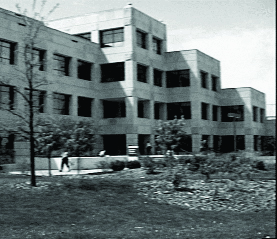
\includegraphics{Images/dc5}

\isucaption{Durham Centre}
\label{mgraph}
\end{figure}

\subsubsection{Parts of the hypothesis}

Here one particular part of the hypothesis that is 
currently being explained is examined and particular
elements of that part are given careful scrutiny.

% Below \subsubsection
% Sectional commands: \paragraph and \subparagraph may also be used

\subsection{Second Hypothesis}

Here one particular hypothesis is explained in depth
and is examined in the light of current literature.

\subsubsection{Parts of the second hypothesis}

Here one particular part of the hypothesis that is 
currently being explained is examined and particular
elements of that part are given careful scrutiny.

\section{Criteria Review}

Here certain criteria are explained thus eventually
leading to a foregone conclusion.

\section{Results}

\section{Conclusion}\label{conclusion3}

The conclusion of the paper goes here.

%%%%
% Reference section comes before the appendix

%\bibliographystyle{acm} % use for numbered citations along with options given in preamble. Look at the main thesis.tex file
\bibliographystyle{apa}
\bibliography{master_bib}

% %\section{Bibliography}
% \bibliographystyle{apa}
% % \vspace{-20pt}
% \begingroup
%     \setlength{\bibsep}{13.2pt}
%     \linespread{1}\selectfont
%     \bibliography{master_bib}
% \endgroup
% \clearpage
% \pagebreak

%%%%%
%% Appendix
% This section may or may not be included
% Chapter 2 shows a double appendix example. Please use A or B as in Appendix A if there are multiple appendix. Use "Appendix A:" before writing the title
% Chapter 3 shows a single appendix example. Use "Appendix:" before writing the title 
\section{Appendix: Appendix title goes here}
If there is an appendix that needs to go with the paper it can be as a section \cite{Aup91}

\subsection{Procedure details}
Details of the paper specific appendix procedures

%\cite{allen}, \cite{bruner} 
\cite{Rad87}
\cite{MOR91}, \cite{Lom73} 
\cite{Lom91}, \cite{Lom92} 
\cite{dB59}
%\chapter{GENERAL CONCLUSION}
\label{future-work}


This is the opening paragraph to my thesis which
explains in general terms the concepts and hypothesis
which will be used in my thesis.

With more general information given here than really
necessary.

\section{Summary And Discussion}

Here initial concepts and conditions are explained and
several hypothesis are mentioned in brief.


\subsection{Hypothesis}

Here one particular hypothesis is explained in depth
and is examined in the light of current literature.

As can be seen in Table~\ref{nothingelse} it is
truly obvious what I am saying is true.

\begin{sidewaystable} \centering
\isucaption{This table shows almost nothing but is a
sideways table and takes up a whole page by itself}
\label{nothingelse}
% Use: \begin{tabular{|lcc|} to put table in a box
\begin{tabular}{lcc} \hline
\textbf{Element} & \textbf{Control} & \textbf{Experimental} \\ \hline
Moon Rings & 1.23 & 3.38 \\
Moon Tides & 2.26 & 3.12 \\
Moon Walk & 3.33 & 9.29 \\ \hline
\end{tabular}
\end{sidewaystable}

\subsubsection{Parts of the hypothesis}

Here one particular part of the hypothesis that is 
currently being explained is examined and particular
elements of that part are given careful scrutiny. \cite{allen}, \cite{bruner}, \cite{struss}


% Below \subsubsection
% Sectional commands: \paragraph and \subparagraph may also be used


%\section{Criteria Review}

%Here certain criteria are explained thus eventually
%leading to a foregone conclusion.

%\bibliographystyle{acm} % use for numbered citations along with options given in preamble. Look at the main thesis.tex file
\bibliographystyle{apa}
\bibliography{master_bib}

% \section{Bibliography}

% \bibliographystyle{apa}
% % \vspace{-20pt}
% \begingroup
%     \setlength{\bibsep}{13.2pt}
%     \linespread{1}\selectfont
%     \bibliography{master_bib}
% \endgroup
% \clearpage
% \pagebreak


%%%%%% bibliographies

%\clearpage
%% \nocite{*}
%\unappendixtitle
%\newpage
%% % \phantomsection
%\addcontentsline{toc}{chapter}{BIBLIOGRAPHY}
%\section*{BIBLIOGRAPHY}
%\bibliographystyle{apa}
%\vspace{-20pt}
%\begingroup
%    \setlength{\bibsep}{14.5pt}
%    \linespread{1}\selectfont
%    \bibliography{master_bib}
%\endgroup

% Renders the citations but does not show the bibliography at the end of the thesis
%\newsavebox\mytempbib
%\savebox\mytempbib{\parbox{\textwidth}{\bibliography{master_bib}}}

\clearpage
\pagebreak

%% Only within chapter appendix is allowed for Journal style writing
%% Appendix1 file from standard thesis template

\appendixtitle 
\appendix


%% Use the following two lines for single appendix
%\unappendixtitle
%\singleappendixtitle

% Please note the appendix can be removed if the thesis does not require an overall appendix

\chapter{ADDITIONAL MATERIAL} 
This is now the same as any other chapter except that
all sectioning levels below the chapter level must begin
with the *-form of a sectioning command.

\section*{More stuff}

Supplemental material.

 % Instruction for single appendix look below
%% An example second appendix from the example thesis thesis.tex.
\chapter{STATISTICAL RESULTS}

This is now the same as any other chapter except that
all sectioning levels below the chapter level must begin
with the *-form of a sectioning command.

\section*{Supplemental Statistics}

More stuff.

\end{document}

% use \isucaption{} for all captions of figures and tables, where the captions are not too long.

% Use \isucaption[]{} with the square brackets for short caption of figure or table that goes into the list of tables and list of figures, and the curly brackets can have long captions which go with the figure/ table.

% IMPORTANT NOTES
% TABLE OF CONTENTS :
% TOPIC 1:  If you need a page break follow the steps below
% step1
% check before which chapter in the table of contents you want a page break
% step 2
% go the folder "body". There open the chapter tex file that you noted needed page break in the table of contents..
% step 3
% insert  \addtocontents{toc}{\protect\newpage} before the first line i.e. before the line \chapter{RESULTS}.

%%%%%%%%%%%%%%
% use \isucaption{} for all captions of figures and tables, where the captions are not too long.

% Use \isucaption[]{} with the square brackets for short caption of figure or table that goes into the list of tables and list of figures, and the curly brackets can have long captions which go with the figure/ table.

%%%%%% Using sub figures 
% %%% In preamble include : \usepackage{subfig}
% \begin{figure}[htbp]
% 	\centering
% 	\subfloat[first caption.\label{fig:2a}]{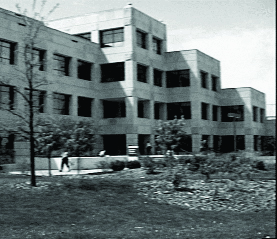
\includegraphics[width=0.2\textwidth]{Images/dc5.jpg}}\hfill
%     \subfloat[second caption.\label{fig:2b}] {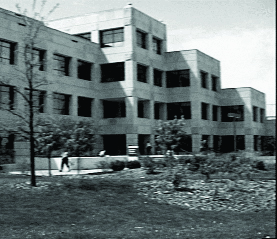
\includegraphics[width=0.2\textwidth]{Images/dc5.jpg}}\hfill
% 	\isucaption{Sub-figure test}
% 	\label{fig:subfigure-test}
% \end{figure}

% Subfloat reference: Fig \ref{fig:2a}

% Figure reference: Fig \ref{fig:subfigure-test}
